
\documentclass[10pt,a4paper]{report}
%\usepackage[latin1]{inputenc}
\usepackage[utf8]{inputenc}
\usepackage{amsmath}
\usepackage{amsfonts}
\usepackage{amssymb}
\usepackage{ragged2e}
\usepackage{graphicx}
\usepackage{fixltx2e}
\usepackage{multicol}
\usepackage{tabularx}
\usepackage{tikz}
\usepackage{hyperref}
\hypersetup{
    colorlinks=true,
    linkcolor=blue,
    filecolor=magenta,      
    urlcolor=blue,
    }
\usepackage{tabularx}
\usepackage{mathtools}
\usepackage{tikz}
\usetikzlibrary{arrows,shapes,automata,petri,positioning,calc}
\usepackage{hyperref}
\usepackage{tikz}
\usetikzlibrary{matrix,calc}
\usepackage[margin=0.5in]{geometry}
% ---- power functions -----% 
\newcommand{\myvec}[1]{\ensuremath{\begin{pmatrix}#1\end{pmatrix}}}
\let\vec\mathbf

\providecommand{\norm}[1]{\left\lVert#1\right\rVert}
\providecommand{\abs}[1]{\left\vert#1\right\vert}
\let\vec\mathbf

\newcommand{\mydet}[1]{\ensuremath{\begin{vmatrix}#1\end{vmatrix}}}
\providecommand{\brak}[1]{\ensuremath{\left(#1\right)}}
\providecommand{\lbrak}[1]{\ensuremath{\left(#1\right.}}
\providecommand{\rbrak}[1]{\ensuremath{\left.#1\right)}}
\providecommand{\sbrak}[1]{\ensuremath{{}\left[#1\right]}}
%-------end power functions----%
\newenvironment{Figure}
  {\par\medskip\noindent\minipage{\linewidth}}
  {\endminipage\par\medskip}
\begin{document}
\begin{figure*}[!tbp]
  \centering
  \begin{minipage}[b]{0.4\textwidth}
   
\includegraphics[scale=0.05]{iitlogo.jpg} 
  \end{minipage}
  \hfill
  \vspace{5mm}\begin{minipage}[b]{0.4\textwidth}
\raggedleft 
\includegraphics[scale=0.3]{nrc.jpg} 
  \end{minipage}\vspace{0.2cm}
\end{figure*}
\raggedright \textbf{Name}:\hspace{1mm} Siva Parvathi Tungala\hspace{3cm} \Large \textbf{Optimization}\hspace{2.5cm} % 
\normalsize \textbf{Roll No.} :\hspace{1mm} FWC22089\vspace{1cm}
\begin{multicols}{2}
\textbf{Problem Statement:}\vspace{2mm}
\justify{A window od fixed perimeter(including the base of the arch) is in the form of a rectangle surmounted by a semi-circle. The semi-circular portion is fitted with coloured glass while the rectangular part is fitted with clear glass. The clear glass transmits three times as much light per square meter as the coloured glass does. What is the ratio of the sides of the rectangle so that the window transmits the maximum light?}
\\
\\
\vspace{4mm}
\textbf{Solution:}
\\
Consider radius(r) of a semi-circle = $x$, also length breadth of a rectangle be $2x$ and $2y$ respectively.\\
Let light trasmit by colour glass = 1 /$m^2$ \\
then, light trasmit by clear glass = 3 /$m^2$\\
Let P be the perimeter of a window, then
\begin{center}
$P=2(2x+2y)+\pi x$
\end{center} 
\begin{align}
\label{eq:one}
P=(4+\pi)x+4y
\end{align}
Let light trasmit by colour glass = 1 /$m^2$ \\
then, light trasmit by clear glass = 3 /$m^2$\\

The function is,
    \begin{align}
    \label{eq:two}
    f(x)=3xP-(12+\frac{5\pi}{2})x^2
    \end{align}
	\textbf{Objective function:}
	\begin{align}
	\max_xf(x)= 3xP-(12+\frac{5\pi}{2})x^2
        \end{align}
	\textbf{constraints:}\\
	\begin{align}
		x \in \mathbb{R}-\{0.1,0.9\} 
	\end{align}
\textbf{Calculation of Maxima using gradient ascent algorithm:}
\justify{Maxima of the above \eqref{eq:two}, can be calculated from the following expression,}
Differentiating  \eqref{eq:six} yields,
\begin{equation}
       \boxed{x_{n+1} = x_n - \alpha \nabla h(x_n)} 
\end{equation}
\begin{align}
\label{eq:six}
f(x) = 3xP-(12+\frac{5\pi}{2})x^2 \\
\nabla f(x) = 3P-(24+5\pi)x
\end{align}
\vspace{1mm}
Taking $x_0=0.1,\alpha=0.0001$ and precision = 0.000001, values obtained using python are:
    \begin{align}
        \boxed{\text{Maxima} =0.656}\\     
    \end{align}
\raggedright\textbf{Theoritical proof:}\\
\vspace{4mm}
Given,
\centering
$f(x)=3xP-(12+\frac{5\pi}{2})x^2$\\
\raggedright Differentiating above equation with respect to x ,
\begin{align}
\frac{df(x)}{dx}=0\\
\label{eq:five}
x=\frac{3P}{24+5\pi}
\end{align}
To find the ratio of sides of a rectangle divide \eqref{eq:one} with x, 
\begin{align}
\frac{P}{x}=\frac{(4+\pi)x+4y}{x}\\
\frac{y}{x}=\frac{1}{4}(\frac{P}{x}-(4+\pi))
\end{align}
By substituting \eqref{eq:five} in above equation we get,
\begin{align}
\frac{y}{x}=\frac{1}{4}(\frac{24+5\pi}{3}-(4+\pi))\\
\frac{y}{x}=\frac{6+\pi}{6}
\end{align}
Thus, the ratio of sides of a rectangle, so that the window transmits the maximum light is,\\
\begin{align}
\frac{x}{y}=\frac{6}{6+\pi}=0.656
\end{align}\\
\raggedright\textbf{Conclusion:}
\justify{1. At first, the given function has been differentiated to find f'(x).
\\
2. Later, the function f(x) is solved by gradient descent algorithm to find maxima and the point at which f(x) is maximum.}\\
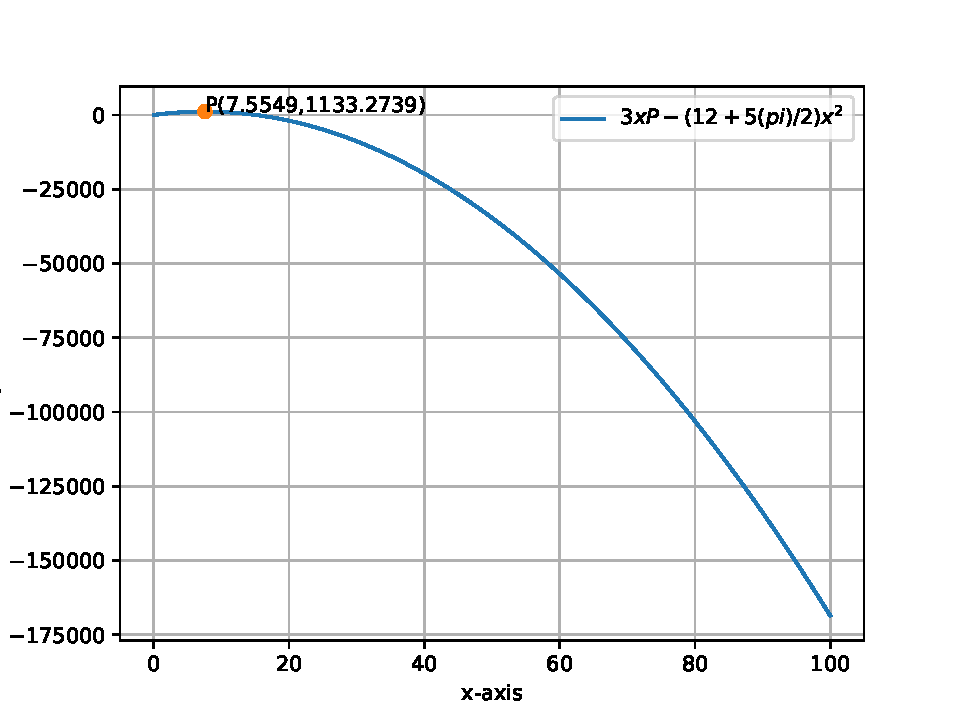
\includegraphics[scale=0.4]{opfig.pdf}\\
Fig.1.  Maxima of light through the window\\
\\Download the code to execute the above problem statement.
\\
\boxed{\href{https://github.com/Sivaparvathi/FWC}{https://github.com/Sivaparvathi/FWC}.}
\end{multicols}
\end{document}
